\chapter{Experiment}\label{Experiment}

Nu we alle achterliggende theorie van het experiment in hoofdstuk \ref{Lectuur} gezien hebben, kunnen we van start gaan. 

Om te weten of er technieken voor Engelse gevoelsanalyse gelijk toepasbaar zijn op het Nederlands en te achterhalen wat juist deze verschillen zijn, hebben we het onderzoek in drie experimenten opgesplitst. De gevoelsanalyse voor deze experimenten bestaat er telkens uit om te bepalen of de gegeven tekst een positive of negatieve emotie uitdrukt. Als eerste experiment vergelijken we de prestaties van de eerder besproken technieken in hoofdstuk \ref{Lectuur} op het Engels met die van het Nederlands. Vervolgens hopen we nog iets meer inzicht te krijgen in de verschillen door een classificatie uit te voeren op basis van Engels en Nederlands geannoteerde woordenlijsten van gevoelens. Als laatste gaan we nog iets dieper in op de Nederlandse gevoelsanalyse en kijken we hoe deze zich gedraagt op data met verschillende onderwerpen.

Voor dat we kunnen beginnen aan de experiment, moeten we eerst over een dataset beschikken waarmee we de algoritmes kunnen trainen en testen. In \ref{De Dataset} gaan we dieper op de dataset. Uiteindelijk is het beschikken over een goede dataset even belangrijk als het beschikken over goede technieken voor dit experiment. 

% Het doel van het experiment is aan de hand van enkele algemene technieken uit te Machine Learning een gevoelsanalyse uitvoeren op Nederlandse tekst, waarbij een algoritme het onderscheid aanleert tussen positief negatief. Het doel is om een algoritme te bekomen dat kan bepalen of een tekst een positieve of negatieve emotie uitdrukt. De prestatie van zo'n algoritme wordt in dit experiment beoordeeld op basis van de classificatieprecisie.  Wanneer het algoritme met een hoge precisie classificeert en bijna alle input correct kan classificeren als positief of negatief, dan spreken we van een goede prestatie. Wanneer de classificatieprecisie rond de 50\% of minder ligt, spreekt men van een slechte prestatie. Een classificatieprecisie van 50\% kan men vergelijken met een classificatiealgoritme dat telkens bij het bepalen van de output een munt gaat opgooien en op basis van kop of munt de output gaat bepalen. Wat neerkomt op het at random bepalen van de output.\\
% %
% Vooraleerst we de resultaten van het experiment bekijken, hebben we het in \ref{De Dataset} over de dataset die we gebruiken. Er is gekozen om gevoelsanalyse uit te voeren op film-, boek- en muziekrecensies. Waarom er is voor gekozen en hoe het verzamelen van de data is verlopen, wordt uitgelegd in deze sectie. In \ref{Naive Bayes Classifier met hetzelfde onderwerp voor trainings- en testset} en \ref{Naive Bayes Classifier met verschillend onderwerp voor trainings- en testset} volgen dan de experimenten en als laatste vatten we alle de bevindingen van het experiment samen in \ref{Conclusie experiment}.

\section{De Dataset}\label{De Dataset}

Als data voor het experiment is er gekozen voor gebruikersrecensies, meer bepaald film-, muziek- en boekrecensies. Recensies bieden alles wat we nodig hebben. Een recensie drukt of wel positieve, negatieve of neutrale mening uit. Maar omdat er meestal een rating aanwezig is bij de review, is het gemakkelijk om de data automatisch te labelen en enkel de positieve en negatieve reviews op te nemen in onze dataset. Verder door het grote aanbod aan reviewsites is het aanbod aan film-, boek- en muziekrecensies enorm en maakt het gebruik van gebruikersrecensies de recensies nog eens toegankelijk en niet te specifiek. 

Voor deze experimenten is de dataset met Engelse filmrecensies afkomstig van een eerder onderzoek door \cite{maas-EtAl:2011:ACL-HLT2011}. De recensies deze website zijn afkomstig van \url{http://www.imdb.com/} en zijn eveneens afkomstig van gebruikers. Voor de Nederlandse reviews waren er geen datasets beschikbaar en moesten deze gescraped worden. De websites \url{moviemeter.nl}, \url{boekmeter.nl} en \url{muziekmeter.nl} vormde de perfecte bron aan informatie om te scrapen. Ze bevatten allemaal toplijsten met films, boeken of muziekalbums waarop vele gebruikers hun persoonlijke mening plaatsen. Verder was er bij iedere recensie duidelijk een score aanwezig, die het mogelijk maakte om de recensies automatische te labelen. Belangrijk om te vermelden is dat zowel bij het labelen van de Engelse als de Nederlandse dataset dezelfde voorwaarden werd gerespecteerd. Enkel hoog gepolariseerde recensies werden beschouwd in de dataset. Onderzoek rond polarisatie classificatie (\cite{maas-EtAl:2011:ACL-HLT2011}) ondersteund deze keuze. Een recensie werd negatief gelabeld als het een score had van $4/10$ of minder. Een positieve labeling werd gegeven aan recensies met een score van $6/10$ of meer.\\

\begin{figure}[h]%
    \centering
    \subfloat{{
\includegraphics[width=10cm]{voorbeeldrecensie} }}%
    \caption{Een voorbeeld van een positieve commentaar op \url{moviemeter.nl}}%
\end{figure}
\newline

Alle Nederlandse recensies zijn afkomstig van de ``All Time Top 250''-toplijst op de betreffende website. Onderstaande linkertabel geeft het aantal verzamelde Nederlandse recensies van ieder onderwerp weer, waarbij een onderscheid wordt gemaakt tussen positief en negatief. Analoog wordt dit in de rechtertabel voor de Engelse recensies weergegeven.\\

\begin{table}[h]
\centering
\begin{tabular}{l|l|l|l|}
\cline{2-4}
                                        & \textbf{Films} & \textbf{Muziek} & \textbf{Boeken} \\ \hline
\multicolumn{1}{|l|}{\textbf{Positief}} & 197358         & 15197           & 146             \\ \hline
\multicolumn{1}{|l|}{\textbf{Negatief}} & 17978          & 3019            & 3719            \\ \hline
\end{tabular}
\caption{Aantal verzamelende recensies} 
\end{table}


Om nog een beter inzicht te krijgen over de dataset geven onderstaande tabellen nog wat extra statistieken weer over de datasets.\\
HIER KOMEN NOG TABELLEN\\

\newpage
\begin{figure}%
    \centering
    \subfloat{{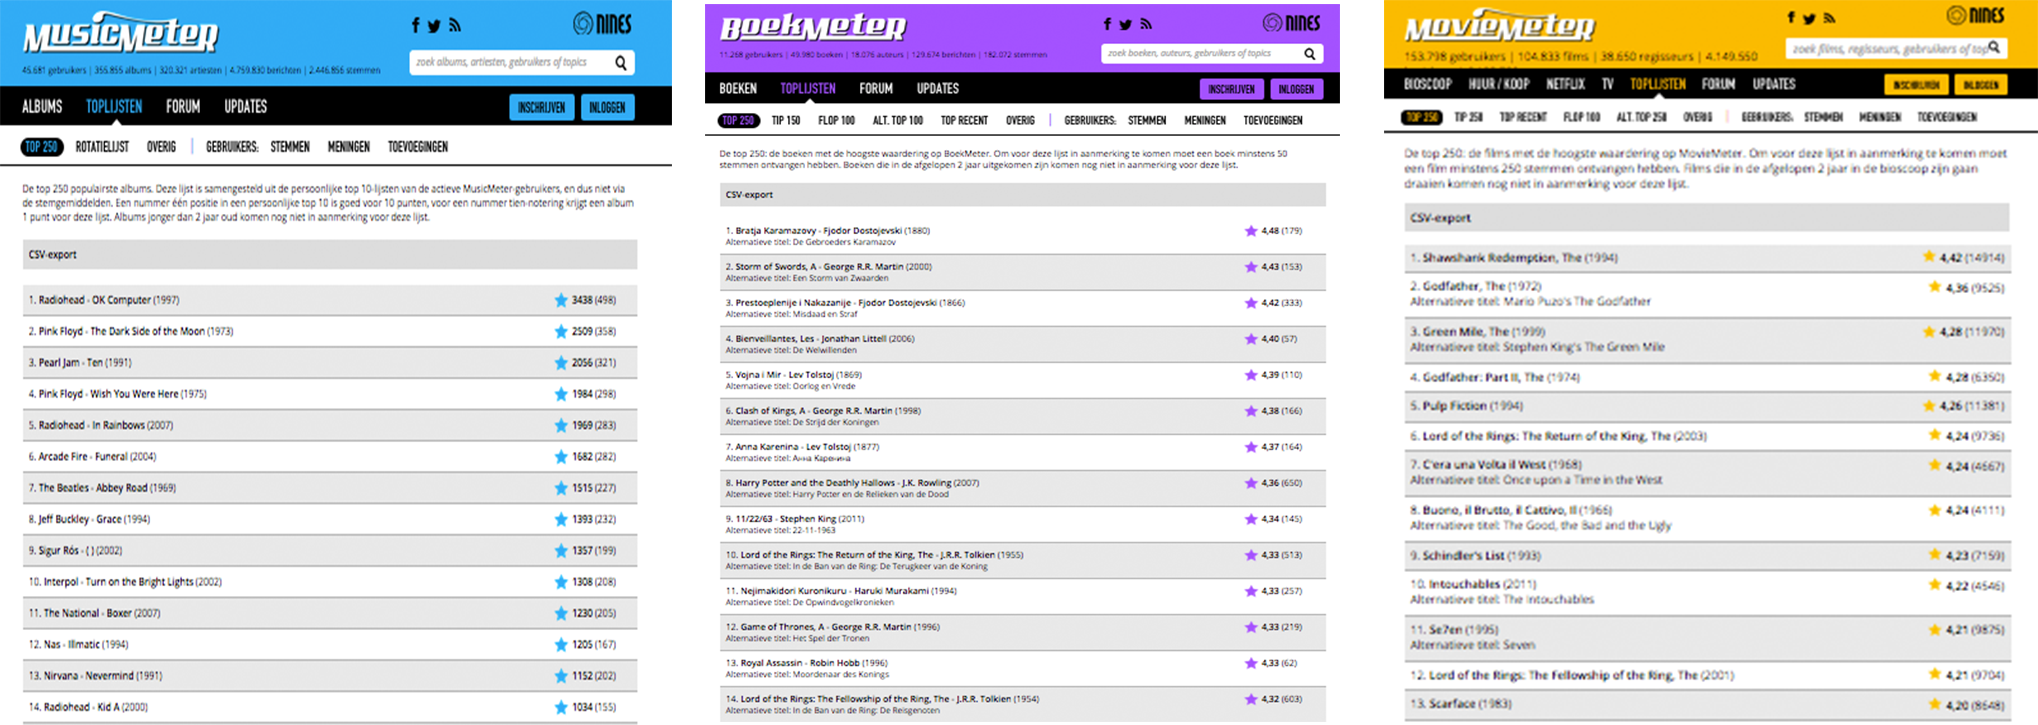
\includegraphics[width=15cm]{toplijsten} }}%
    \caption{de ``All Time Top 250''-toplijsten op de websites}%
\end{figure}


Voor het tweede experiment hebben we als woordenlijsten het \textit{Opinion lexicon} gebruikt, dat voor het eerst werd samengesteld door \cite{hu2004mining}. De woordenlijsten bestaan uit een lijst met negatieve en een lijst met positieve woorden. De lijsten bevatten in totaal ongeveer 6800 woorden en zijn enkel in het Engels verkrijgbaar. De Nederlandse woordenlijsten hebben we verkregen door de Engelse lijsten te vertalen met behulp van Google vertalen.\\

Onderstaande tabel geeft weer hoe de woordenlijsten zich tegenover elkaar verhouden.\\
HIER KOMT NOG EEN TABEL\\

% Wat meteen opvalt is dat er aanzienlijk minder positieve boekrecensies verzameld zijn. Hier zullen we rekening mee moeten houden tijdens het experiment. Voor de andere categorie\"en zijn de positieve recensies in grotere aantallen aanwezig dan de negatieve recensies, wat te maken heeft met dat we de ``All Time Top 250''-toplijst gebruiken voor zowel films, boeken als muziek als databron.

\section{Methodologie}\label{Methodologie}
\section{Engelse gevoelsanalyse versus Nederlandse Gevoelsanalyse}\label{Engelse gevoelsanalyse versus Nederlandse Gevoelsanalyse}
Als eerste experiment vergelijken we Engelse gevoelsanalyse met die van Nederlandse gevoelsanalyse. Concreter gaan we de geziene technieken in  hoofdstuk \ref{Lectuur} gebruiken om filmrecensies naar positieve en negatieve recensies te classificeren en vergelijken we deze prestaties voor het Engels en het Nederlands. De prestatie wordt bepaald op basis van de precisie waarmee de classifier de recensies classificeert. De precisie die we opnemen voor een classifier wordt bepaald door het gemiddelde te nemen van 30 runs. Bij iedere run wordt er een ongetrainde classifier getraind met een trainingsset en wordt de precisie getest door het classificeren van de testset. In dit experiment bestaat iedere trainingsset uit 6000 samples en testset uit 2000 samples. Ook zijn ze telkens at random samengesteld en gebalanceerd. Dit wil zeggen dat de datasets telkens voor $1/2$ uit positieve en $1/2$ negatieve recensies bestaan en wanneer men deze at random zou classificeren, men een precisie baseline van $50\%$ krijgt.\\

Voor de datasets gebruiken de besproken Engelse en Nederlandse filmrecensies uit \ref{De Dataset}.  
Onderstaande tabel geeft de belangrijkste resultaten weer van het experiment. In bijlage A vindt men de volledig tabel met resultaten.\\

HIER RESULTATEN TABEL

\section{Classificatie op basis van geannoteerde woordenlijsten}\label{Classificatie op basis van geannoteerde woordenlijsten}


Om meer inzicht te krijgen over de verschillen in de gevoelsanalyse bij de twee talen, voeren we nog een tweede experiment uit. Bij dit experiment gaan we heel eenvoudig en intu\"itief te werk. We kijken hoe de classificatie verloopt, wannneer we enkel geannoteerde woordenlijsten met gevoelens in beschouwing nemen. Er wordt voor iedere recensie gekeken, hoeveel woorden van de recensie voorkomen in de positieve lijst en hoeveel in de negatieve. De lijst met de meest overeenkomstige woorden geeft aan of de recensie positief of negatief moet worden geclassificeerd.\\
Voor de woordenlijsten gebruiken we de eerder vermeldden woordenlijsten uit \ref{De Dataset}. De classificatie zelf testen we op de Engelse en Nederlandse filmrecensies.\\
Onderstaande tabel geeft de resultaten van de classificatie weer met als precisie het gemiddelde van 30 runs en een testset van 2000 samples random en gebalanceerd samengesteld.

HIER TABEL RESULTATEN


\section{Analyseren van de resultaten}\label{Analyseren van de resultaten}

\section{Onderwerpgevoeligheid van Nederlandse Gevoelsanalyse}\label{Onderwerpgevoeligheid van Nederlandse Gevoelsanalyse}

Nu we weten welke methode goed presteert op het Nederlands en welke niet, kunnen we er nog iets dieper ingaan op Nederlandse gevoelsanalyse. De voorgaande experimenten zijn altijd uitgevoerd op filmrecensies en hadden goede prestaties. Het is interessant om eens te kijken of de voorgaande technieken onderwerp gevoelig zijn of niet. Concreet voor dit experiment onderzoeken we enkel de beste presterende techniek uit \ref{Engelse gevoelsanalyse versus Nederlandse Gevoelsanalyse}, namelijk de Naive Bayes Classifier in combinatie met Term weighting en het verwijderen van stopwoorden. We kijken hoe deze techniek presteert wanneer we het trainen en testen met recensies over hetzelfde onderwerp en hoe het presteert met een verschillend.  Als datasets nemen we film- , muziek en boekrecensies. De prestatie van de classifiers is telkens de gemiddelde classificatieprecisie van 30 runs, waarbij de trainingsset uit 6000 samples bestaat en de testset uit 2000 samples. 

Onderstaande kruistabel met classificatieprecisies vat de belangrijkste resultaten van het experiment samen. De volledige resultaten vindt men in bijlage B. Merk op dat men hier ook de controle op over- of onderfitting vindt. Over- en onderfitting zijn symptomen bij machine learning waarbij men de classifier over of ondertrained. Voor de volledigheid hebben we deze grafieken in de bijlage toegevoegd.    

HIER KOMT EEN TABEL

Als laatste hebben nog de confusion matrixen van het experiment. Een confusion matrix geeft weer hoeveel recensies er juist en fout geclassificeerd zijn. 

\begin{table}[h]
\centering
\setlength\tabcolsep{4pt}
\begin{minipage}[t]{0.48\textwidth}
\centering
\begin{tabular}{lll}
                                 & \textbf{P}               & \textbf{N}               \\ \cline{2-3} 
\multicolumn{1}{l|}{\textbf{P'}} & \multicolumn{1}{l|}{43\%} & \multicolumn{1}{l|}{6\%} \\ \cline{2-3} 
\multicolumn{1}{l|}{\textbf{N'}} & \multicolumn{1}{l|}{18\%} & \multicolumn{1}{l|}{31\%} \\ \cline{2-3} 
\end{tabular}
\caption{Gemiddelde confusion matrix in percent voor een Naive Bayes Classifier, waar trainings- en testset over hetzelfde onderwerp gaan}
\end{minipage}%
\hfill
\begin{minipage}[t]{0.48\textwidth}
\centering
\begin{tabular}{lll}
                                 & \textbf{P}               & \textbf{N}               \\ \cline{2-3} 
\multicolumn{1}{l|}{\textbf{P'}} & \multicolumn{1}{l|}{32\%} & \multicolumn{1}{l|}{18\%} \\ \cline{2-3} 
\multicolumn{1}{l|}{\textbf{N'}} & \multicolumn{1}{l|}{21\%} & \multicolumn{1}{l|}{29\%} \\ \cline{2-3} 
\end{tabular}
\caption{Gemiddelde confusion matrix in percent voor een Naive Bayes Classifier, waar trainings- en testset over een verschillend onderwerp gaan} 
\end{minipage}
\end{table}

\begin{table}[h!]
\centering
\begin{tabular}{c >{\bfseries}r @{\hspace{0.7em}}c @{\hspace{0.4em}}c @{\hspace{0.7em}}l}
  \multirow{10}{*}{\parbox{1.1cm}{\bfseries\raggedleft eigelijke\\ waarde}} & 
    & \multicolumn{2}{c}{\bfseries voorspelde waarde} & \\
  & & \bfseries p & \bfseries n  \\
  & p$'$ & \MyBox{Waar}{Positief} & \MyBox{Vals}{Negatief}  \\[2.4em]
  & n$'$ & \MyBox{Vals}{Positief} & \MyBox{Waar}{Negatief} \\
\end{tabular}
\caption{Illustratie van de confusion matrix} 
\end{table}

